\Subsection{ХАРАКТЕРИСТИКА КОЛЕБАНИЯ МАДДЕНА--ДЖУЛИАНА}

Принято описывать климатические моды с помощью специальных индексов, которые упрощают анализ данных явлений. Существует множество индексов, описывающих КМД, но наиболее распространённым является Real-time Multivariate MJO index (RMM), введённый в \cite{Wheeler_Hendon_2004}. Индекс RMM рассчитывается на основе потока уходящей длинноволновой радиации (outgoing longwave radiation, OLR) и скорости зонального ветра на 200 и 850 гПа (такие давления достигаются на высотах в 10-11 и 1-2 км соответственно). Набор трёх таких переменных, взятых на широтно-долготной сетке 2.5\textdegree\texttimes2.5\textdegree, позволяет выделить паттерны, характерные для КМД, как в атмосферной циркуляции (которая характеризуется зональными ветрами), так и в глубокой конвекции (которая описывается OLR).

КМД всегда происходит совместно с климатической изменчивостью, происходящей на прочих временных и пространственных масштабах. Поэтому все три параметра, на основе которых рассчитывается КМД, сперва обрабатываются с целью удаления большей части изменчивости, не связанной с КМД. После этого производится осреднение всех трёх параметров в полосе 15\textdegree~с.~ш. – 15\textdegree~ю.~ш., что приводит к тому, что для каждого дня имеется три набора данных, каждый из которых обладает длиной 144. Такие три набора данных объединяются вместе и формируют 432-размерный вектор, для которого выделяются эмпирические ортогональные функции (ЭОФ). ЭОФ для физического процесса --- такие взаимно ортогональные пространственные паттерны, рассчитываемые из данных, что с их помощью можно устроить разложение сложного процесса на относительно простые части. Первая ЭОФ выбирается таким образом, что объясняет большую возможную часть дисперсии данных, вторая ЭОФ выбирается таким образом, что объясняет большую возможную часть дисперсии оставшихся данных и так далее \cite[Гл. 6]{Zhang_et_al_2020} (более строго процесс вычисления ЭОФ и ГК будет описан в разделе \ref{subsec:2-6}). Временные коэффициенты для различных ЭОФ называются главными компонентами (ГК). Первые две ГК для вышеописанного набора данных составляют индекс RMM и обозначаются как RMM1 и RMM2.

Физически RMM1 описывает колебание конвекции над Морским Континентом (Maritime Continent), под которым подразумевается обширный район (по долготе от 90\textdegree~в.~д. до 150\textdegree~в.~д. и по широте между 20\textdegree~с.~ш. и 10\textdegree~ю.~ш.) между Индийским и Тихим океаном, включающим Индонезийский архипелаг, острова Борнео, Новая Гвинея, Филиппинские острова и окружающие моря; RMM2 отвечает за колебание конвекции над Индийским океаном (см. рис. \ref{fig:wh04_fig1}). Принято иллюстрировать состояние КМД как точку на плоскости (RMM1, RMM2), которая называется фазовой и изображена на рис. \ref{fig:rmm_diagram}, на котором отмечена стрелкой типичная траектория состояния КМД на плоскости (RMM1, RMM2). На рис. \ref{fig:wh04_fig7} показаны реальные траектории состояний КМД на фазовой плоскости, видно, что они сильно изменчивы, но в среднем совпадают с движением по окружности против часовой стрелки.

\begin{figure}[t]  
    \centering
    \begin{subfigure}{.49\textwidth}
		\centering
		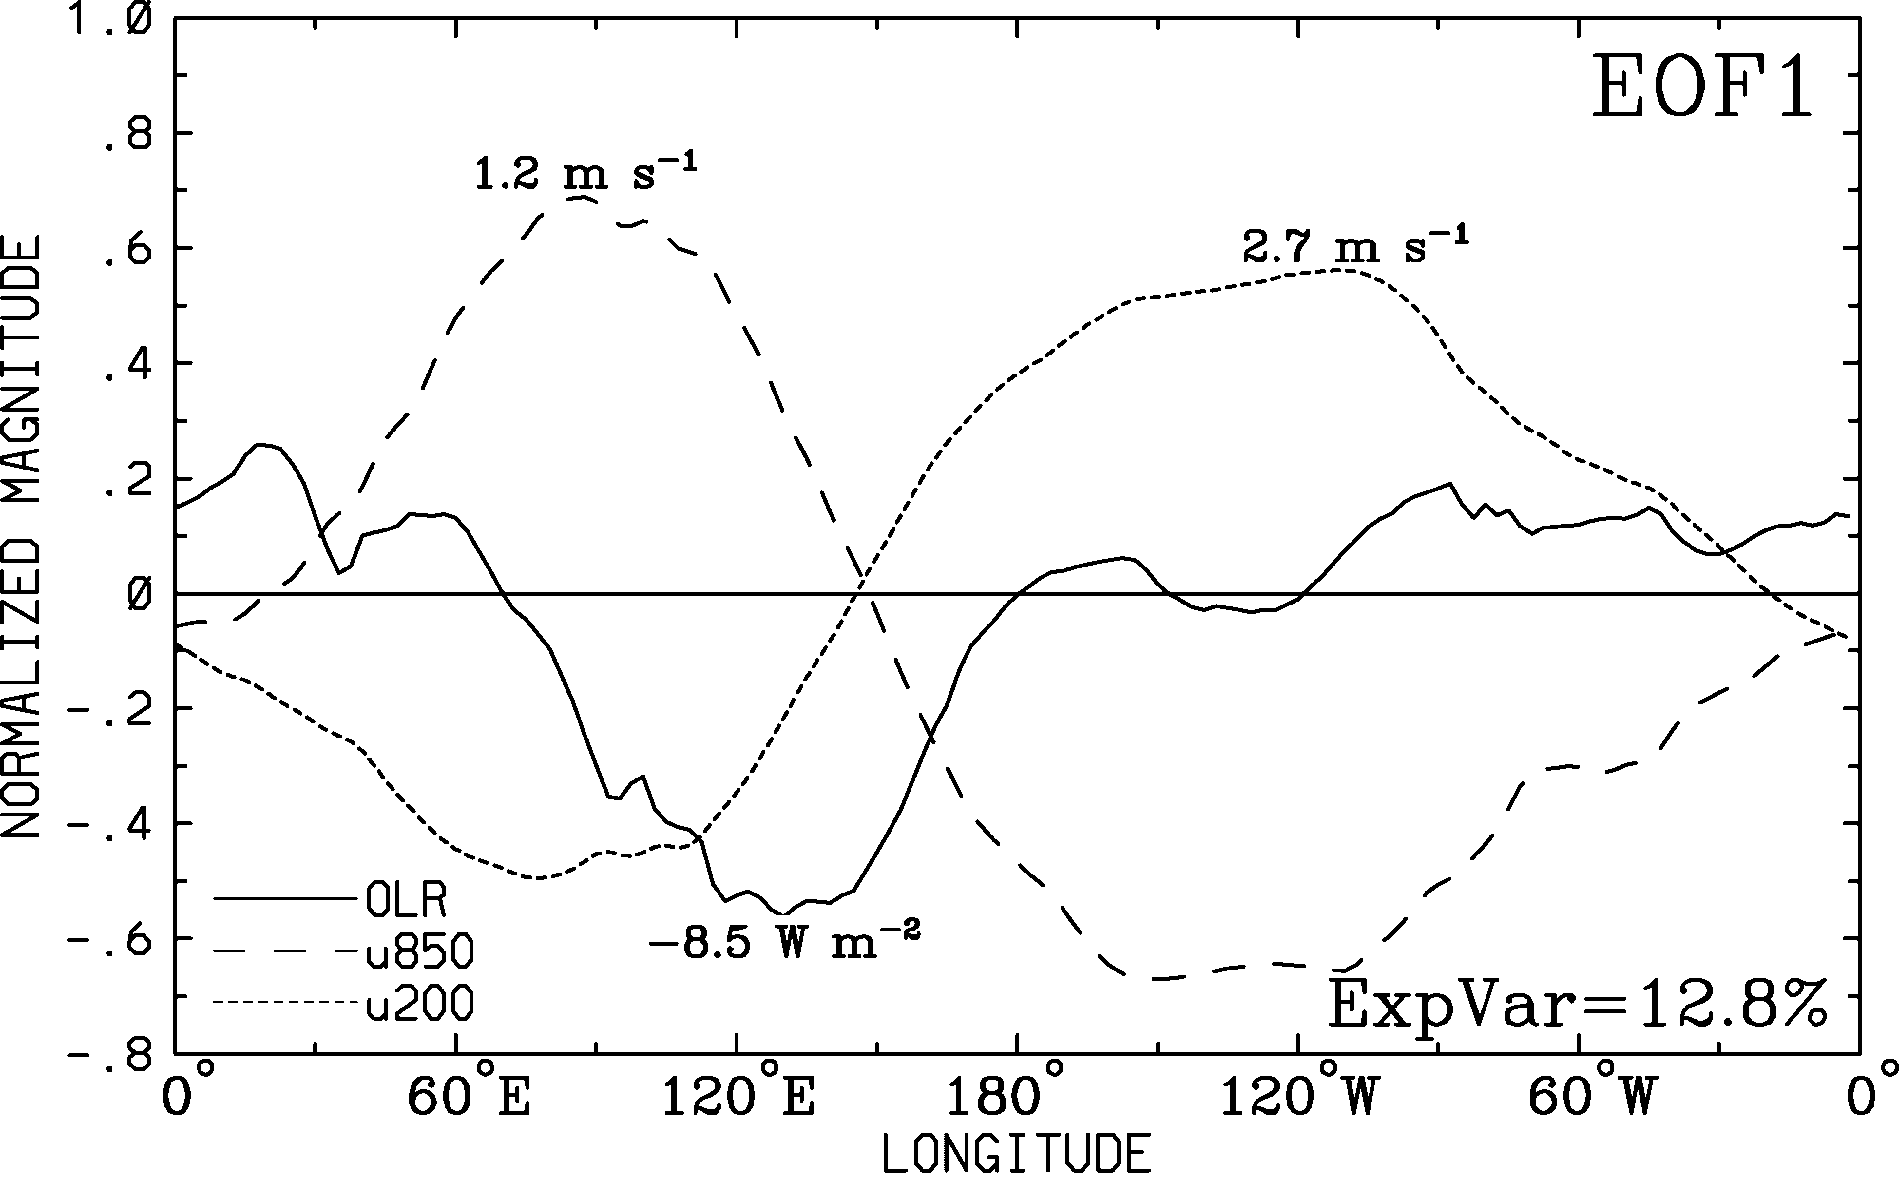
\includegraphics[width=\textwidth]{figures/wh04_fig1_eof1.png}
    \end{subfigure}
    \hfill
    \begin{subfigure}{.49\textwidth}
		\centering
		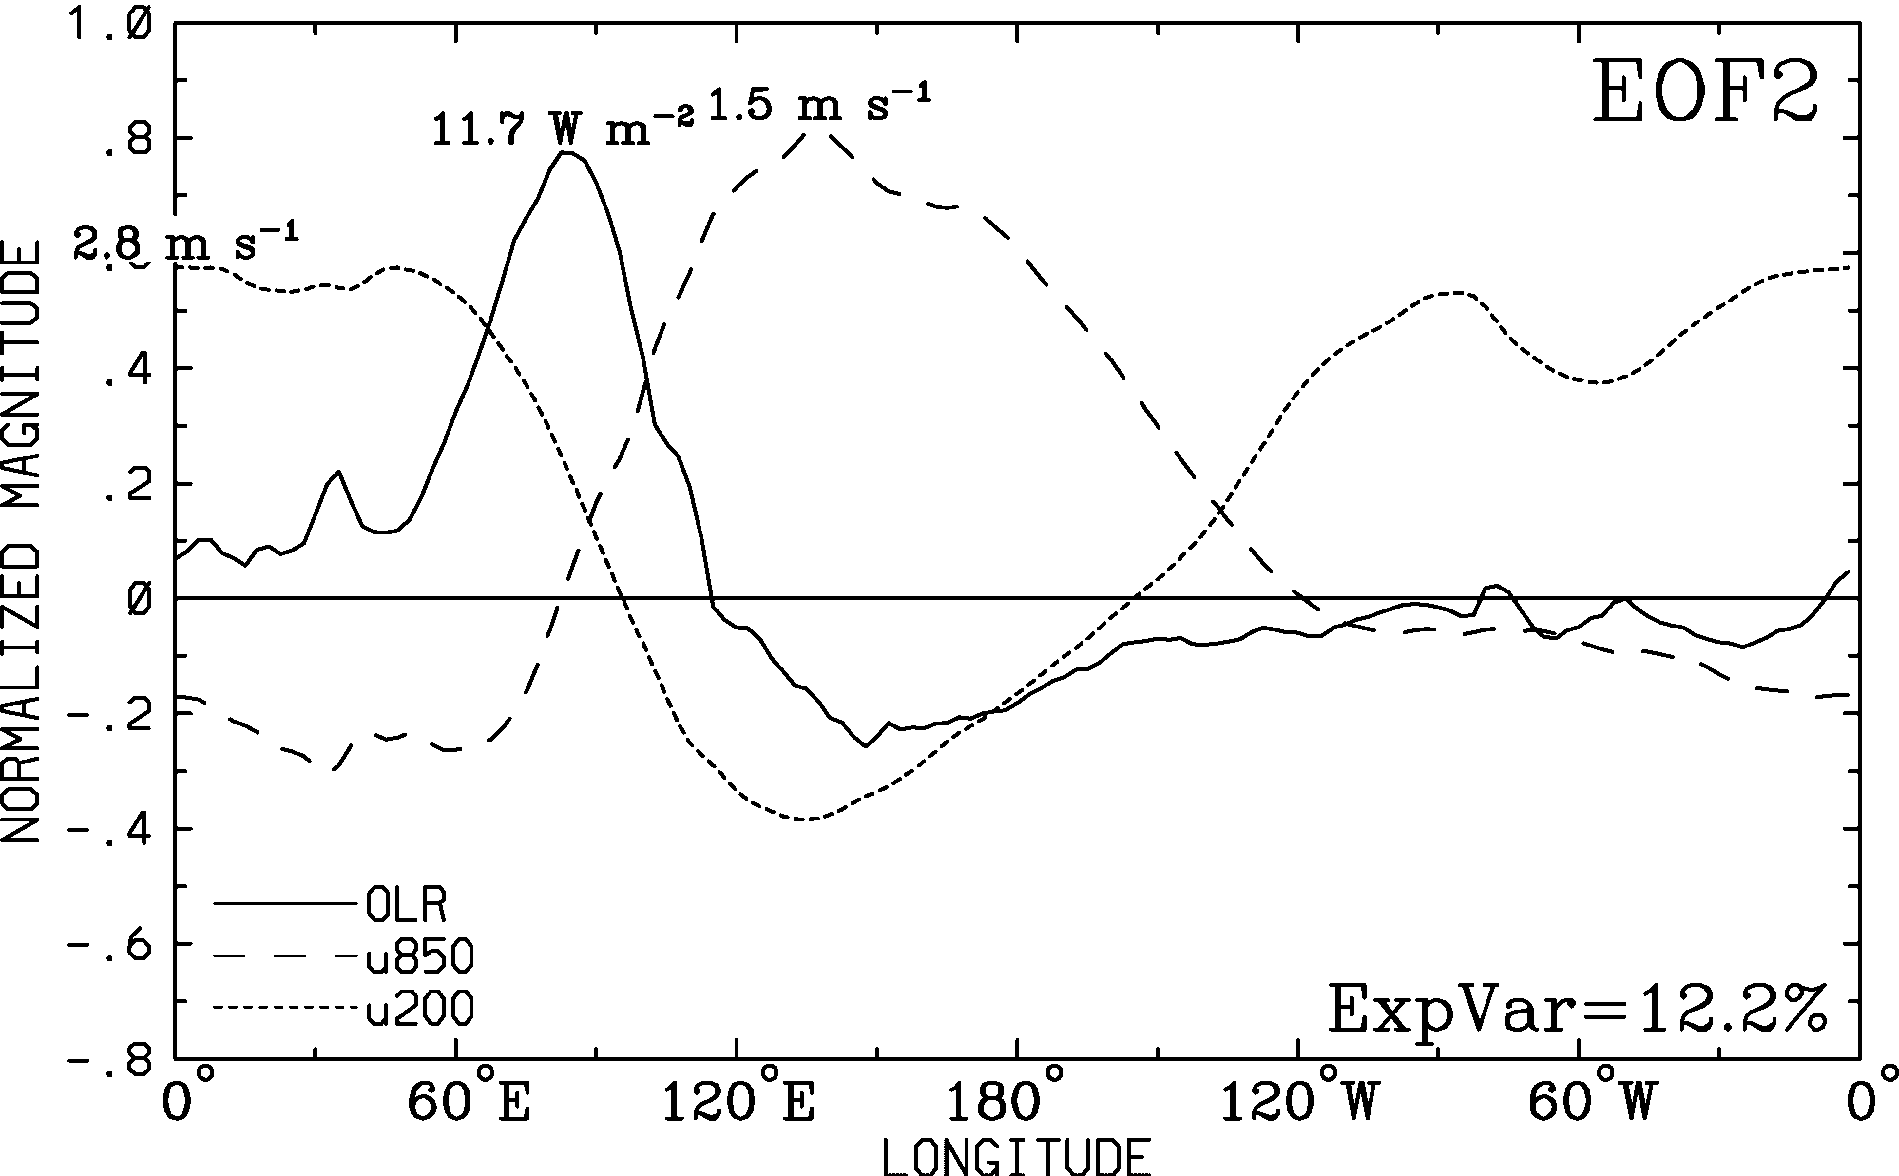
\includegraphics[width=\textwidth]{figures/wh04_fig1_eof2.png}
    \end{subfigure}
    \caption{Долготная структура первых двух ЭОФ, получаемых при вычислении индекса RMM. Непрерывные кривые обозначают OLR и описывают паттерны глубокой конвекции, характерные для КМД. Взято из \cite[рис. 1]{Wheeler_Hendon_2004}.}
	\label{fig:wh04_fig1}
\end{figure}

\begin{figure}
    \centering  
    \begin{subfigure}[tb]{.45\textwidth}
		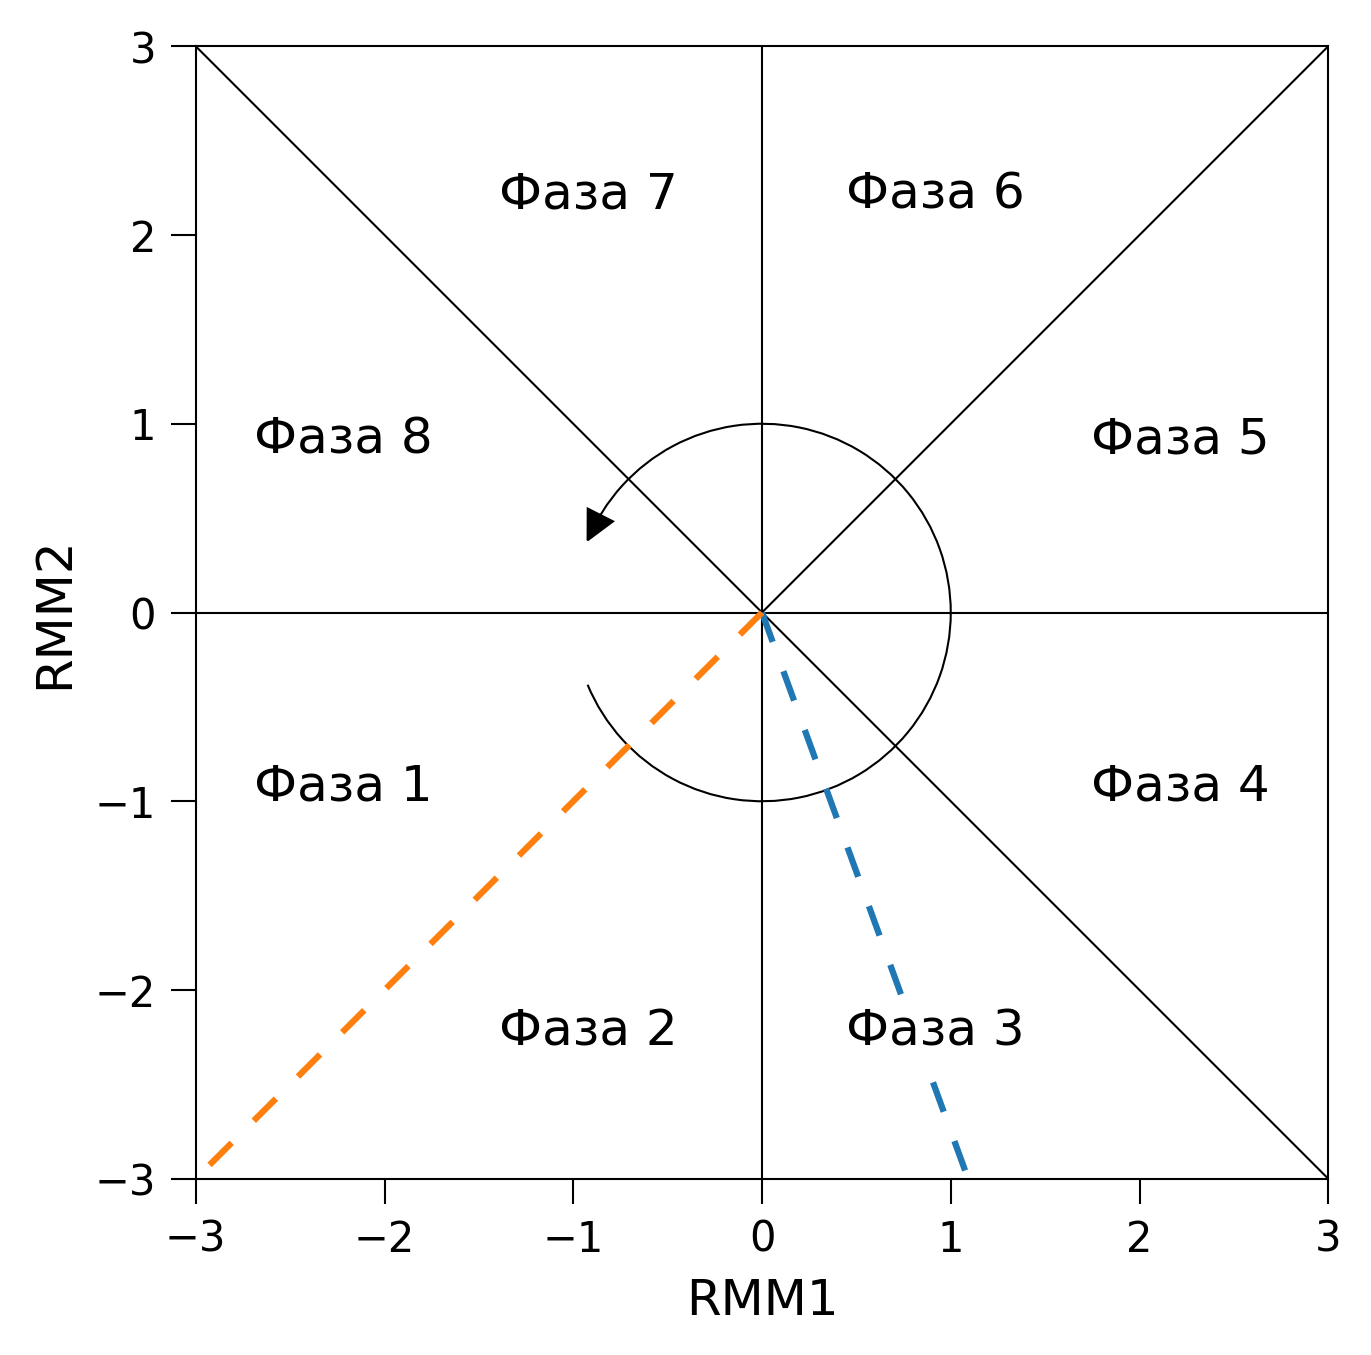
\includegraphics[width=\textwidth]{figures/rmm_diagram.png}
		\caption{}
		\label{fig:rmm_diagram}
	\end{subfigure}
	\hfill
	\begin{subfigure}[tb]{.45\textwidth}
		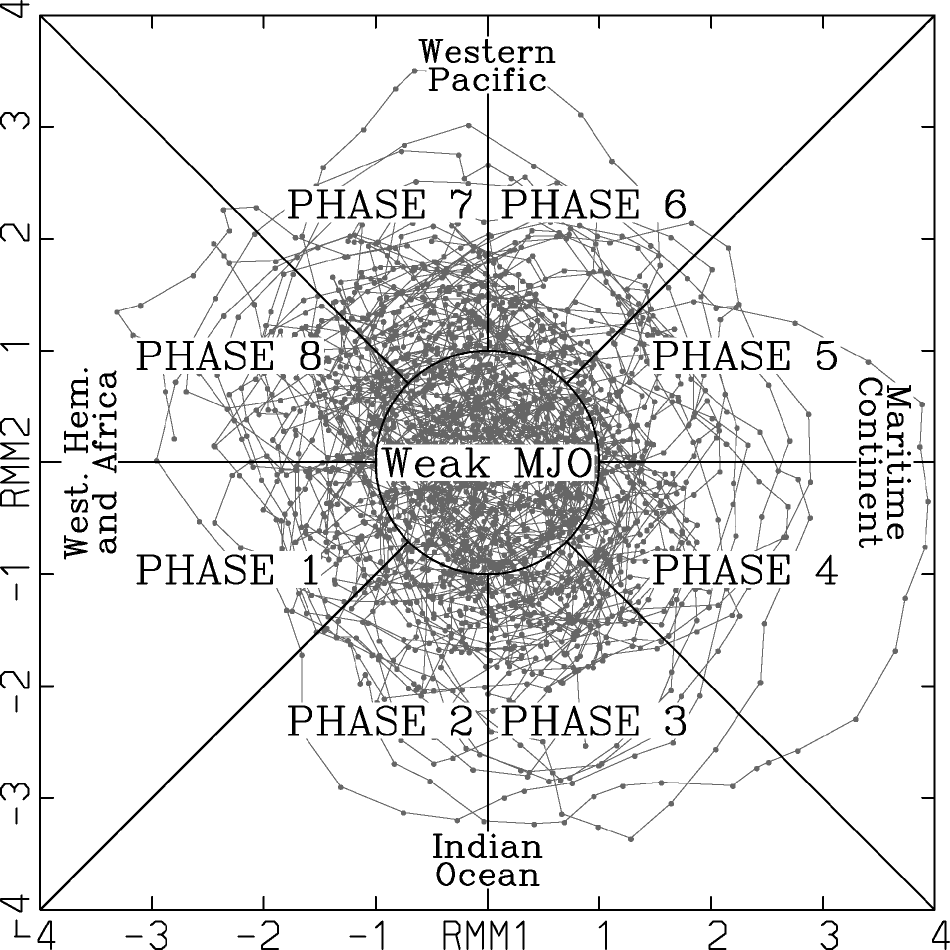
\includegraphics[width=\textwidth]{figures/wh04_fig7.png}
		\caption{}
		\label{fig:wh04_fig7}
	\end{subfigure}
    \caption{(a): Разбиение фазовой плоскости индекса RMM на восемь секторов, которые определяются как восемь фаз КМД. Закрученная стрелка схематично обозначает типичную траекторию точки в течение одного цикла КМД. Пунктрирными линиями отмечены направления на плоскости (RMM1, RMM2), дающие наибольшую корреляцию с моделируемым ИП (голубая линия) и с измеренным в Антарктике в дни хорошей погоды ГП (оранжевая линия). (b): Траектория состояний КМД в зимние месяцы с 1974 по 2003 год на плоскости (RMM1, RMM2). Взято из \cite[рис. 7]{Wheeler_Hendon_2004}.}
    \label{fig:rmm_planes}
\end{figure}

В настоящем работе использовались данные индекса RMM за период 1980--2020 годов, которые были взяты с веб-сайта Австралийского бюро метеорологии (\url{http://www.bom.gov.au/climate/mjo /}).
